\documentclass[a4paper]{article}

\usepackage[utf8]{inputenc}
\usepackage[russian]{babel}
\usepackage{pgfplots}
\usepackage{pgfplotstable}
\usepackage{amssymb}
\usepackage{amsmath}
\usepackage{graphicx}
\textheight=24cm
%
\textwidth=16cm
%
\oddsidemargin=0pt
%
\topmargin=-1.5cm


\title{Задание №3. Дифференциальные уравнения в частных производных}
\author{Попыкина Алёна, Козлов Алекснадр}
\date{16 мая 2020 года}

\begin{document}
\maketitle
    Решали численными методами уравнение $u_t = u_{xx} + \delta(x)$ с граничными условиями $u_x(-1, t) = u_x(1, t) = 0$ и начальным условием $u(x, 0) = 0$. Аппроксимировав производные и дельта-функцию, получили следующую явную разностную схему:
    \begin{equation}\label{Numerical}
        \bar u_n= u_n+ \frac{\Delta t}{{\Delta x}^2}\{ u_{n+1}- 2u_n +u_{n-1}\} + \Delta t f_n,
    \end{equation}
    где
    \begin{equation}
        f(x) =
        \begin{cases}
         & \frac1{\Delta x},\ \text{если $x \in (-2\Delta x,\ 2\Delta x )$}\\
         & 0,\ \text{если $x \bar \in (-2\Delta x,\ 2\Delta x )$}
        \end{cases}
    \end{equation}
    Численная аппроксимация дельта-функции является собой размытый пик, площадь под которым равна единице.\par
    
    Реализация данной схемы дала решение, график котогоро приведён ниже. Так как вычислительная возможность графической библиотеки ${\tt {\bf pgfplots}}$ ограничена, то график построен не по всем точкам, что может выдать программа, а только по 5000 из них (выводилась каждая пятая точка по времени). Поэтому график может быть несколько неточным и резким.\par
    Из графика видно, что граничные условия, как и начальные, выполняются.\\
    Для проверки было найдено численное решение данного уравнения. Получен ответ:
\[
 U = \sum_{k=1}^{\infty} \frac{1-e^{-(k\pi)^2t}}{(k\pi)^2} \cos(k\pi x) + \frac{t}{2}
\]
Его график представлен ниже. Как видно решения численное и аналитическое хорошо соотносятся.
    \begin{figure}[h]
        \noindent\centering{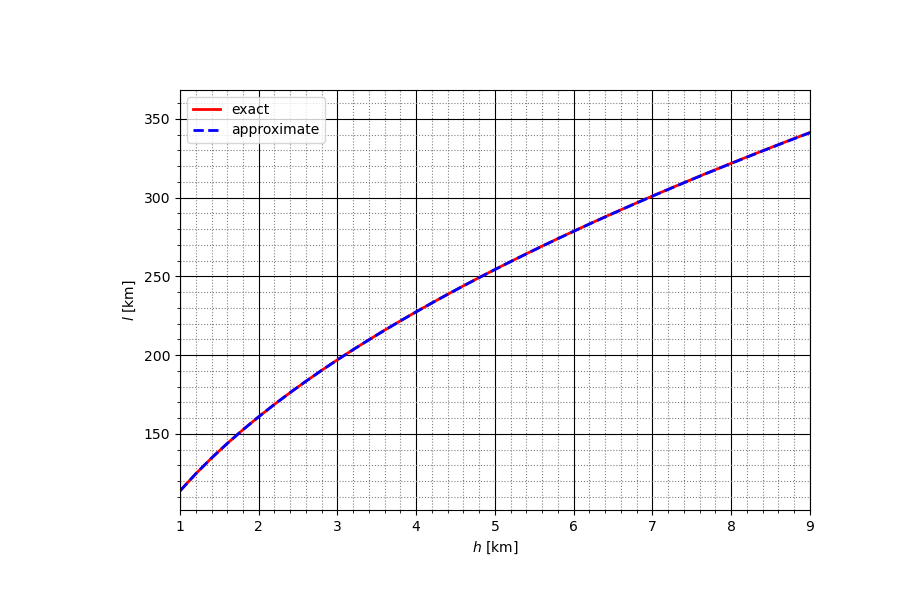
\includegraphics[width = 15 cm]{1.jpg}}
        \caption{Аналитическое решение, учтены первые 50 членов ряда}
        \label{graph1}
    \end{figure} 
\begin{tikzpicture}
    \begin{axis}[
	xlabel=$x$,
	ylabel=$t$,
	zlabel={$u(x,t)$},
	title={Numerical solution of $u_t = u_{xx} + \delta(x) $},
	width = 130 mm
    ]
	\addplot3[surf,
  mesh/interior colormap={blueblack}{color=(blue) color=(red)},
  samples=31,    
  miter limit=1, 
  mesh/interior colormap thresh=0.1,
  colormap/blackwhite, 
  domain=0:1]
        plot table [
            x=X,
            y=T,
            z=U
        ]{data.txt};
    \end{axis}
\end{tikzpicture}
\end{document}
